%%%%%%%%%%%%
%
% $Autor: Wings $
% $Datum: 2019-03-05 08:03:15Z $
% $Pfad: PushButton $
% $Version: 4250 $
% !TeX spellcheck = en_GB/de_DE
% !TeX encoding = utf8
% !TeX root = filename 
% !TeX TXS-program:bibliography = txs:///biber
%
%%%%%%%%%%%%

% Structure
\chapter{Built-in Push Button}\index{Push Button! Built-in Push Button}

\section{General}

A push button is a simple switch mechanism used to control various devices and processes. It is typically made of hard materials like plastic or metal.
The surface of a push button is designed to be easily depressed or pushed by the human finger or hand. When you press a push button, it either closes or opens an electrical circuit. 

In industrial and commercial applications, push buttons can be linked together so that pressing one button releases another. Emergency stop buttons, often with large mushroom-shaped heads, enhance safety in machines and equipment. Pilot lights are sometimes added to push buttons to draw attention and provide feedback when the button is pressed. Color-coding is common to associate push buttons with their specific functions (e.g., red for stopping, green for starting). \cite{DIN:13850}

%\Mynote{cite books, applications, board\\ image of the board}






\section{Built-in Push Button}

The Arduino Nano 33 BLE Sense features an onboard push button. This button is a simple electrical switch that can be activated by pressing it. When you press the button, it completes an electrical circuit. The push button is designed for user interaction and can be used for various purposes.

The built-in button \PYTHON{BUTTON\_B} is connected with pin 11.\index{Pin!Pin 11} Using the function \PYTHON{pinMode(BUTTON\_PIN, INPUT\_PULLUP)} the pin is declared as an input. As can be seen in the sketch, pressing the button can be used to trigger actions; typical actions include switching on an LED, changing modes, or initiating sensor readings.
Overall, the push button provides a convenient way to interact with the Arduino Nano 33 BLE Sense and create responsive projects. \cite{Arduino:2023a,Arduino:2023,ArduinoNano33Manual:2022}


\bigskip



\begin{center}    
    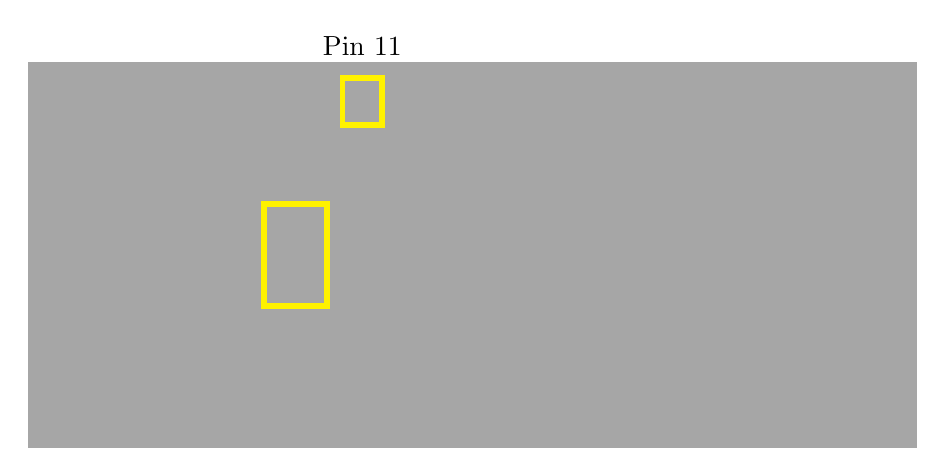
\begin{tikzpicture}
        %\node at (0,0) (Board) {\includegraphics{Arduino/Nano33BLE/Nano33BLESense}};
        
        \ArduinoNanoTikz;
        
        \fill[gray, opacity=0.7] (-11.2,-0.2) rectangle (0.1,4.7);
        
        \coordinate (A) at (-8.2,1.6);
        \coordinate (B) at (-7.4,2.9); 
        
        
        \coordinate (C) at (-7.2,3.9);
        \coordinate (D) at (-6.7,4.5);  
        
        \def\cliparea{(C) rectangle (D); (A) rectangle (B); }  
        
        \begin{scope}
            \clip (A) rectangle (B);
            
            \ArduinoNanoTikz
            
            %\node at (0,0) (Board) {\includegraphics{Arduino/Nano33BLE/Nano33BLESense}};
            
        \end{scope}
        
        %        \fill[ArduinoColor] (C) rectangle (D);
        %         \fill[gray!30] ({-8.16-0.195},4.145) rectangle ++(0.39, 0.39); 
        %        \draw[fill=gray!30,gray!30] (-8.145,4.143) circle(0.195); 
        %        \draw[fill=gray!60,gray!60] (-8.145,4.143) circle(0.165); 
        %        \fill[white,white](-8.145,{4.143+0.39}) circle (0.1275);
        
        \draw[yellow,line width=2pt] (A)  rectangle (B);
        \draw[yellow,line width=2pt] (C)  rectangle (D);
        
        \node (P25) at (-6.95, 4.9) {Pin 11};
    \end{tikzpicture}    
    
    
    
    \captionof{figure}{Arduino Nano 33 BLE Sense's built-in Push Button  with Pin 11}  
\end{center}

\section{Specification}

The built-in button is a small white button  and connected to pin 11.\index{Pin!Pin 11}

\begin{description}
    \item [Built-in Button:] \PYTHON{BUTTON\_B =  11u}
\end{description}

If the pin is declared as input in the function \PYTHON{setup}, then it can be used.

%\Mynote{cite data sheet, power consumption?}

The pin 11 must be defined as an input in the function \PYTHON{setup} by setting \PYTHON{pinMode (11, INPUT\_PULLUP)}, otherwise the button cannot be read.

\medskip 


The pin 11 can also be used otherwise. Then the button is not in use. \cite{Arduino:2023a,Arduino:2023,ArduinoNano33Manual:2022}

%\Mynote{What happen if there is another button at the pin? Both in use?}


\begin{itemize}
  \item cite data sheet
  \item Circuit Diagram
\end{itemize}


\section{Simple Code}


As soon as the button is connected, it can be used. It is not necessary to install a special library. Programming takes place in two steps:

\begin{enumerate}
    \item In the first step, the pin is configured in the function \PYTHON{setup}:
    
    {
        \captionof{code}{Defining the built-in button's pin as an input.}
        \begin{Arduino}
            pinMode(BUTTON_B, INPUT_PULLUP)   
        \end{Arduino}
    }
    \item In the second step, the button can be used in the function \PYTHON{loop}. To read in the value, use the function \PYTHON{digitalRead}:
    
    {
        \captionof{code}{Read the built-in button's state}
        \begin{Arduino}
            buttonState = digitalRead(BUTTON_B);
        \end{Arduino}
    }
    
\end{enumerate}




\section{Tests}


The simplest test is the flashing of an LED for 2 seconds, if the button is pressed, see sketch \ref{Nano:BuiltinButtonTest}.

{
    \captionof{code}{Simple sketch to test the push button and the built-in LED}\label{Nano:BuiltinButtonTest}
    \ArduinoExternal{}{../../Code/Nano33BLESense/Test/TestPushButton.ino}
}




\section{Simple Application}


In the sketch \ref{Nano:TestButtonInterrupt}, pressing the push button triggers an interrupt. The interrupt function is defined, changing the state of a flag. If the flag has the value \PYTHON{true}, the built-in LED is switched on for 2 seconds. After the 2 seconds, the built-in LED is switch off and the value of the flag is set to \PYTHON{false} back. \cite{ArduinoInterrupt:2019}


{
    \captionof{code}[Simple sketch connects the push button with an interrupt.]{Simple sketch connects the push button with an interrupt. Here, pushing the built-in button is handled by an interrupt. Then the built-in LED switch on for 2 sec.}\label{Nano:TestButtonInterrupt}
    \ArduinoExternal{}{../../Code/Nano33BLESense/Test/TestPushButtonInterrupt.ino}
}

\bigskip

This is just a simple example. The variable \PYTHON{BUTTON\_B} is already defined, so the assignment is not necessary. The command \PYTHON{delay} should be avoided in an Arduino sketch. Instead, variables of the type \PYTHON{elapsedMillis} should be used.



\section{Further Readings}

\begin{itemize}
  \item Boxall, John: \textsl{Arduino Workshop - A Hands-On Introduction with 65 Projects}. No Starch Press, 2021. \cite{Boxall:2021}
  \item Vo{\"s}, Andreas: \textsl{Volumio mit Drehgebern erweitern}. Make Magazin, 2024. \cite{Voss:2024}
  \item K\"uhnel, Claus: \textsl{Arduino - Das umfassende Handbuch}. Rheinwerk Verlag GmbH, 2024. \cite{Kuehnel:2024}
\end{itemize}

